\documentclass[a4paper,12pt]{report}


% EXTRA PACKAGES

\usepackage{multirow}
\usepackage{array}
\usepackage{wrapfig, caption, tabu, caption, subcaption, verbatim}
\usepackage{rotating}
\usepackage{textcomp}
\usepackage{listings}
\usepackage{xcolor}
\usepackage{amsmath,amsfonts}
\usepackage{tikz}
\usetikzlibrary{shapes.geometric, arrows}

\usepackage[flushleft]{ragged2e}

\lstset{
	frame=tb, % draw a frame at the top and bottom of the code block
	tabsize=3, % tab space width
	showstringspaces=false, % don't mark spaces in strings
	numbers=left, % display line numbers on the left
	commentstyle=\color{green}, % comment color
	keywordstyle=\color{blue}, % keyword color
	stringstyle=\color{red}, % string color
	backgroundcolor=\color{black!5},
	basicstyle=\small,
	breaklines=true,
	postbreak=\raisebox{0ex}[0ex][0ex]{\ensuremath{\color{red}\hookrightarrow\space}}
}


%%%%%%%%%%%%%%%%%%%%%%%%%%%%
% LINE SPACING
\newcommand{\linespacing}{1.5}
\renewcommand{\baselinestretch}{\linespacing}
%%%%%%%%%%%%%%%%%%%%%%%%%%%%


%%%%%%%%%%%%%%%%%%%%%%%%%%%%
% BIBLIOGRAPHY STYLE
\bibliographystyle{unsrtnat}
\usepackage[numbers,sort&compress]{natbib}
%\usepackage{natbib}
% \bibliographystyle{plain} for [1], [2] etc.
%\bibliographystyle{plain}
%%%%%%%%%%%%%%%%%%%%%%%%%%%%


%%%%%%%%%%%%%%%%%%%%%%%%%%%%
% OTHER FORMATTING/LAYOUT DECLARATIONS
% Graphics
\usepackage{graphicx,color}
\usepackage{epstopdf}
\usepackage[british]{babel}
% The left-hand-side should be 40mm.  The top and bottom margins should be
% 25mm deep.  The right hand margin should be 20mm.
\usepackage[a4paper,top=3cm,bottom=3cm,left=4cm,right=2.5cm,headsep=10pt]{geometry}
\flushbottom
% Pages should be numbered consecutively thorugh the main text.  Page numbers
% should be located centrally at the top of the page.
\usepackage{fancyhdr}
\fancypagestyle{plain}{
	\fancyhf{}
	% Add "DRAFT: <today's date>" to header (comment out the following to remove)
	%\lhead{\textit{DRAFT: \today}}
	%
	%\chead{\thepage}
	\cfoot{\thepage}
	\renewcommand{\headrulewidth}{0pt}
}
\pagestyle{plain}
%%%%%%%%%%%%%%%%%%%%%%%%%%%%


%%%%%%%%%%%%%%%%%%%%%%%%%%%%
% ANY OTHER DECLARATIONS HERE:

%%%%%%%%%%%%%%%%%%%%%%%%%%%%


%%%%%%%%%%%%%%%%%%%%%%%%%%%%
% HYPERREF
\usepackage[colorlinks,pagebackref,pdfusetitle,urlcolor=black,citecolor=black,linkcolor=black,bookmarksnumbered,plainpages=false]{hyperref}
% For print version, use this instead:
%\usepackage[pdfusetitle,bookmarksnumbered,plainpages=false]{hyperref}
%\usepackage{backref}
%\renewcommand{\backrefpagesname}{Cited on}
%%%%%%%%%%%%%%%%%%%%%%%%%%%%

%%%%%%%%%%%%%%%%%%%%%%%%%%%%
% BEGIN DOCUMENT
\begin{document}
%%%%%%%%%%%%%%%%%%%%%%%%%%%%


%%%%%%%%%%%%%%%%%%%%%%%%%%%%
% PREAMBLE: roman page numbering i, ii, iii, ...
\cfoot{\thepage}
\pagenumbering{roman}

%%%%%%%%%%%%%%%%%%%%%%%%%%%%


%%%%%%%%%%%%%%%%%%%%%%%%%%%%
%% TITLE PAGE: The title page should give the following information:
%%	(i) the full title of the thesis and the sub-title if any;
%%	(ii) the full name of the author;
%%	(iii) the qualification aimed for;
%%	(iv) the name of the University of Sussex;
%%	(v) the month and year of submission.
\thispagestyle{empty}

\begin{figure}
	\centering
	
\includegraphics[width=6cm]{HW_logo}
\end{figure}	
\vskip40mm
\begin{center}
% TITLE
\huge\textbf{Investigation and Implementation of Biologically Inspired Flocking Behaviour in Swarm Robotics}
\vskip7mm
% AUTHOR
\Large\textbf{Helmi Fraser}
\vskip1mm
\Large\textit{H00152077}
\normalsize
\end{center}
\vfill
\begin{flushleft}
\large
% QUALIFICATION
An Honours report submitted for the degree of:\\
BEng in Robotics, Autonomous and Interactive Systems \\
Heriot-Watt University	\\
Supervisor: Dr. Matthew W. Dunnigan
% DATE OF SUBMISSION
%March 2017
\end{flushleft}		
%%%%%%%%%%%%%%%%%%%%%%%%%%%%


%%%%%%%%%%%%%%%%%%%%%%%%%%%%
% DECLARATIONS
\chapter*{Declaration}
I, Helmi Fraser

State that this work submitted for assessment is my own and expressed in my own words. Any uses made within it of works of other authors in any form (eg. ideas, figures, text, tables) are properly acknowledged at their point of use. A list of the references employed is included.
% ADDITIONAL DECLARATIONS HERE (IF ANY)

\vskip5mm
Signature:
\vskip20mm
% AUTHOR
Helmi Fraser
%%%%%%%%%%%%%%%%%%%%%%%%%%%%

%%%%%%%%%%%%%%%%%%%%%%%%%%%%
% ACKNOWLEDGEMENTS
\chapter*{Acknowledgements}
\renewcommand{\baselinestretch}{\linespacing}
\small\normalsize
% ACKNOWLEDGEMENTS HERE:
\begin{flushleft}
I would like to thank my supervisor, Dr Matthew Dunnigan, for providing me with project related support and advice. I would also like to thank Mohamed, my library friend, for lending me his industry experience and advising me on valuable software engineering practices. 

Last but certainly not least, I would like to thank my loving girlfriend, Victoria, for keeping me motivated and focused and without whom my time as an undergraduate student would not have been the same.
\end{flushleft}

%%%%%%%%%%%%%%%%%%%%%%%%%%%%

\chapter*{Synopsis}


This project investigates the behaviour and mechanics of natural swarm systems such as social insects, schools of fish and flocks of birds and applies this to an group of robots. This collective of robots, also termed a swarm, is capable of quickly aggregating and moving as a cohesive unit.


%%%%%%%%%%%%%%%%%%%%%%%%%%%%
% TABLE OF CONTENTS, LISTS OF TABLES & FIGURES
%\newpage
\pdfbookmark[0]{Contents}{contents_bookmark}
\tableofcontents



%%%%%%%%%%%%%%%%%%%%%%%%%%%%
% MAIN THESIS TEXT: arabic page numbering 1, 2, 3, ...
%\newpage
\pagestyle{fancy}
\cfoot{\thepage}
\clearpage
\pagenumbering{gobble}
\flushleft
%%%%%%%%%%%%%%%%%%%%%%%%%%%%


%\chapter*{Synopsis}


This project investigates the behaviour and mechanics of natural swarm systems such as social insects, schools of fish and flocks of birds and applies this to an group of robots. This collective of robots, also termed a swarm, is capable of quickly aggregating and moving as a cohesive unit.

\clearpage
\pagenumbering{arabic}

\chapter{Introduction}
\label{chap:Introduction}

Nature has shown that it is often beneficial for animals to live and travel with groups of similar animals. In predatory social animals, they are often called packs and in prey animals the nomenclature varies from animal to animal, from flocks to herds, to schools. Indeed, humans are not exempt from this, with early humans coming together to form sizeable groups. 

It is thought that the reason for this is that it is evolutionarily advantageous. For example, predators hunting in a group allow the hunting of far bigger prey animals than themselves, which provides an easier source of sustenance at the cost of being forced to share their bounty. \cite{social-predation} Conversely, other animals - like birds, fish, sheep and so on - group together in an effort to avoid such predations. These animals have developed antipredator adaptations through evolution because there is safety in numbers. Acting as a unit can provide protection and decrease the likelihood of an attack or fatality.

As can be seen, the concept of \textit{flocking} and group behaviour is highly beneficial within natural systems. If this can be understood fully and leveraged for artificial systems, it can bring with it many of the benefits it has shown in nature. This is especially suited for implementation within robotics, specifically the field of \textit{swarm robotics}.

Swarm robotics is a relatively new field of multi-robotics, in which the aim is to co-ordinate a large number of robots in a decentralized manner, similar to biological systems found in nature. The crux of a swarm system is feedback: a swarm cannot operate without some sort of feedback to its constituent individual agents. Systems may contain direct or indirect methods of feedback, either agent-agent communication or agent-environment-agent communication. In addition to this, swarm systems promote \textit{scalability}, by emphasizing a large number of agents.

Where this project is concerned, flocking is used to demonstrate the applicability of biologically inspired techniques when applied to a swarm of robots. Flocking behaviour and the techniques that are used in its operation can be especially useful when working with a group of robots.

\section{Aim}
This project aims to model, implement and explore the swarming behaviour exhibited in biological systems such as social insects, birds, schools of fish and bacteria. This will be achieved by developing a robot controller that will operate on every individual agent within a simulated robot swarm. The resulting global behaviour will then be compared against those found in natural systems.


\section{Objectives}
 This project's objectives are:-

\begin{enumerate}
	\item To understand the theory and concepts behind a swarm system, be they natural or artificial.
	\item To develop a robot controller which exhibits \textit{flocking} behaviour, based on the techniques of self-organising swarm systems.
	\item To evaluate the developed system under dynamic environmental conditions and stressors.
	%\item To analyse the resulting behaviour and compare the similarity and effectiveness of the controller against other solutions and biological equivalents.
\end{enumerate}

\section{Relevance}

From an engineering perspective, mimicking natural systems could provide better solutions to a multitude of problems across various industries. One way that is gaining major interest from academics and the industry alike is the application of swarm robotics.

In a world where there exists an increasing reliance on ``smart'' products and artificial intelligence, distributed computing and distributed robotics is becoming more and more commonplace. In effect, the world is a multi-agent system and there exists a need for artificial systems to be able to effectively operate in it.

Swarming theory can be applied to any problem that would benefit from having multiple agents solving it, such as search and rescue, subsea and space exploration and autonomous vehicles. 

The potential use of the implementation of these algorithms in a commercial application is plentiful. For example, foraging and dispersal techniques can see major use in optimizing both disaster relief/rescue and agriculture. Flocking techniques can be applied to autonomous vehicles - which are predicted to significantly increase in market share in the coming years - in order to improve collision detection and efficiency. Of course, real life systems will be more nuanced and will need further development, but a proof of concept in the lab is vital to developing an engineer's understanding of these technologies further.



\chapter{Literature Review}
\label{chap:LiteratureReview}

In this chapter, an analysis of previous work completed in the field of swarm robotics is provided, as well as an outline of the theoretical concepts concerning the techniques applied during this project.

\section{Biologically Inspired Computation and Engineering}

Nature has provided examples of outwardly complex biological systems which are often efficient, fluid
and resilient to partial breakdowns. Colonies of ants are able to forage for food and build large, complex
structures. Fireflies are able to synchronize their flashing with one another. Flocks of birds and schools of fish exhibit fluid
and efficient group movement. In the majority of cases, nature has achieved these despite utilizing very little to
no communication between individual creatures and in the absence of a higher level director or supervisor.
The animals react only to environmental stimuli, either the strength or type of pheromones detected in the environment in the case of
ants (termed \textsl{stigmergy}) or the positions of other individuals in the case of fish and birds. For example, it has been shown that over time, the velocity of a flock of birds converges to a state where each individual has equal velocity. \cite{cucker-smale}

This is defined as \textsl{emergent behaviour}, the rise of previously unpredicted and complex behaviour through the interaction of simple rules.

Researchers have attempted to replicate this in an artificial system via various means. For example, Bojinov et. al (2000) demonstrated how simple, local sensory rules can produce complex and useful structures in metamorphic robots. \cite{Bojinov2000}  Metamorphic, or modular, robots are a relatively new concept which can be described as "a robot that is composed of modules that are all identical". \cite{Yim} In their paper, Bojinov et. al explored the use of purely \textit{local} rules and interactions to develop control algorithms which enabled a Proteo robot to accomplish some otherwise difficult and complex tasks. Such tasks include forming three dimensional structures, locomotion and dynamic adaptation.

Previous work on this front has utilised an exact, a-priori definition of the configuration of the robot, calculated via algorithms that use heuristics. \cite{metricsrob} These algorithms all require knowledge of the problem, the environment and the desired shape before hand, which in a real world setting is not always feasible.  What makes the work of Bojinov et. al interesting is that their algorithm does not aim to produce a pre-defined shape, rather it aims to produce a shape with the desired \textsl{properties} needed to solve the problem at hand. In this way, the algorithm produced is robust to unknowns, noise or changes in the environment, in a similar manner to how animals can adapt to changes in their environment.

From an engineering perspective, mimicking these systems could provide better solutions to a multitude
of problems across various industries. One way that is gaining major interest from academics and the
industry alike is the application of swarm robotics. Swarm robotics is a relatively new field of multi-
robotics, in which the aim is to co-ordinate a large number of robots in a decentralized manner, similar to
the natural systems mentioned previously. In order to carry out this project, a thorough understanding of
the concepts and mechanisms that underpin swarm robotics systems will need to be achieved, as well as
a strong working understanding of various tools used in their implementation such as simulation software
and higher level programming.

\section{Artificial Intelligence}
Something about aim

\section{Collective and Swarm Intelligence}
Aims and objectives are different, somehow


\chapter{Methodology}
\label{chap:Methodology}

\section{Hardware}
\subsection{E-puck robots}
E-pucks
\subsection{Alternatives}
Others

\section{Software}
\subsection{Webots simulator}
\subsubsection{Concepts}

\subsection{C++ programming language}

\chapter{Implementation}
\label{chap:Implementation}

\section{Design}

\subsection{System Diagram}
E-pucks
\subsection{Control Equations}
Others

\subsection{Software Architecture}

\section{Code Implementation}

\subsection{Libraries and dependencies}

\subsection{Low level}

\subsection{High level}

\subsection{Behavioural}

\chapter{Evaluation}
\label{chap:Evaluation}

Within this section, the evaluation process of this project will be outline, as well as the resulting experimental results.

Evaluating this swarm system successfully poses several questions:-

\begin{enumerate}
	\item Can the system be described as exhibiting flocking behaviour in line with the definition of a swarm system?
	\item How quickly does the system form a state of flocking?
	\item Does the swarm have the ability to form splinter groups?
	\item Can these splinter groups amalgamate to form one flock?
	\item How well does the system deal with failure?
	\item Is the swarm system scalable?
\end{enumerate}

Answering these questions will provide a thorough evaluation of the system's success. To that end, an experiment will be conducted for each question, with the aim of gathering data to make conclusions.
\clearpage

\section{Testing}

\subsubsection{Experiment 1: Can the system be described as exhibiting flocking behaviour in line with the definition of a swarm system?}

With regard to robotics, \citeauthor{VanDykeParunak2004} defined swarming as ``useful self-organization of multiple entities through local interactions''. \cite{VanDykeParunak2004} Following this definition, an assessment of the system can be made.

The ability of the system to self-organise and move as a group can be tested by executing the program and observing the simulation. The cohesiveness of the swarm can be validated by capturing both the GPS data and the number of detected robots in the swarm and comparing these.

The swarm may be evaluated further by comparing the behaviour of the system to the behaviour exhibited by natural systems and observing the similarities and differences.

\subsubsection{Experiment 2: How quickly does the system form a state of flocking?}

This can be measured by recording the current heading of the robot and the number of neighbours each robot detects, at every simulation time step. Once this data has been gathered, an analysis can be made.

\subsubsection{Experiment 3: Does the swarm have the ability to form splinter groups?}

This question can be answered by executing a simulation where some members of the swarm are segregated from the others and observing the behaviour over time. Also, positional and neighbourhood data can be gathered to further validate the conclusion.

\subsubsection{Experiment 3: Can these splinter groups amalgamate to form one flock?}

This question and the last can be tested during the same experiment. Once separate groups have been formed, the segregation can be removed and the behaviour of the two groups analysed.

\subsubsection{Experiment 4: How well does the system deal with failure?}

Failure within a swarm can be defined in a number of ways. The main point of failure, however, are the agents themselves. In this case it can be simulated by powering down robots during execution of the program. This will test to see if the system can adapt to changing circumstances. 

\subsubsection{Experiment 5: Is the swarm system scalable?}

One of the defining features of a robot swarm is the system's scalability. This can be easily tested through the addition of more agents to the swarm and observing the system's behaviour. GPS and neighbourhood data can also be gathered and these can be compared with different swarm sizes for analyses. 
\clearpage
\section{Results and Analysis}
\label{section:results}

Upon conducting the experiments outlined in the previous section, the results as well as a discussion of the findings are presented here.

\subsection{Experiment 1}

\begin{figure}[!h]
	\centering
	\begin{minipage}{.5\textwidth}
		\centering
		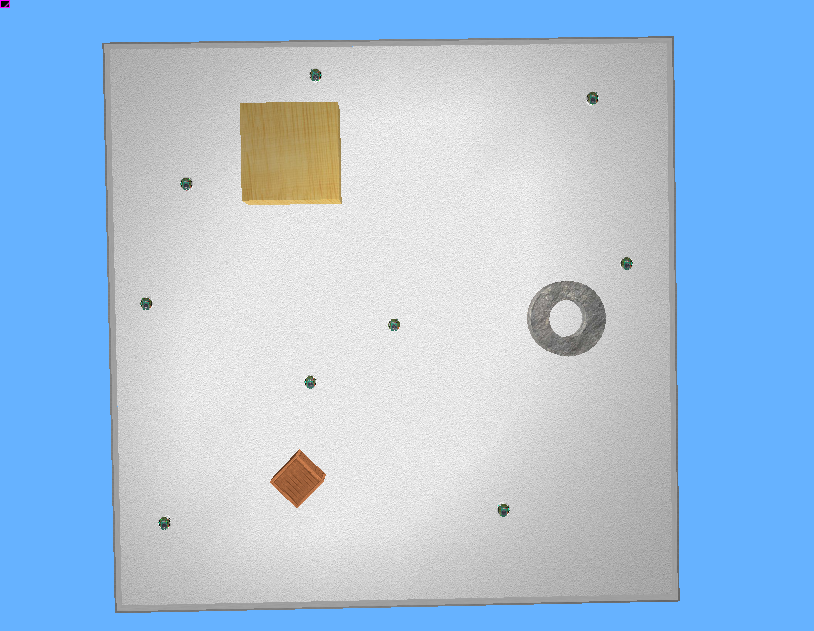
\includegraphics[width=.75\linewidth]{swarm_test_1}
		\caption*{t = 0s}
		\label{fig:sw1}
	\end{minipage}%
	\begin{minipage}{.5\textwidth}
		\centering
		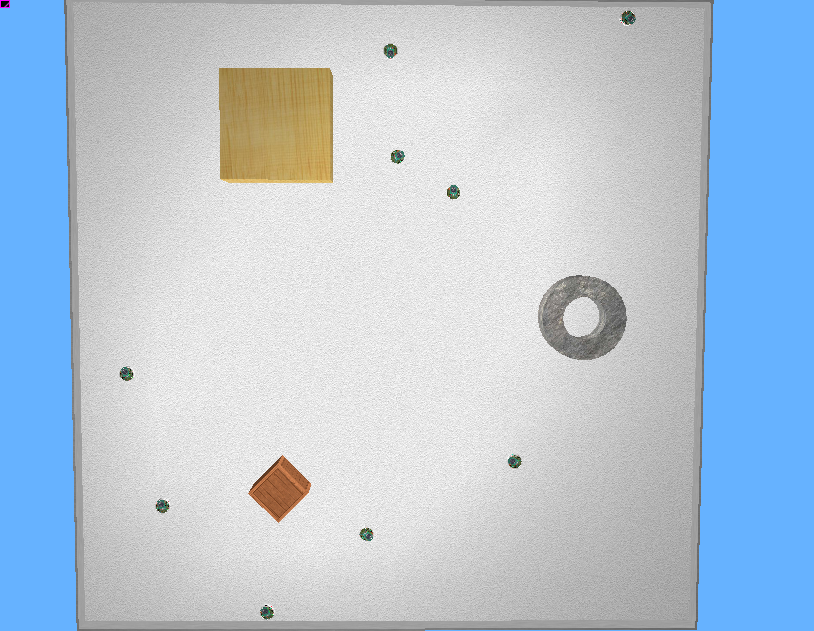
\includegraphics[width=.75\linewidth]{swarm_test_2}
		\caption*{t = 10s}
		\label{fig:sw2}
	\end{minipage}
	\begin{minipage}{.5\textwidth}
		\centering
		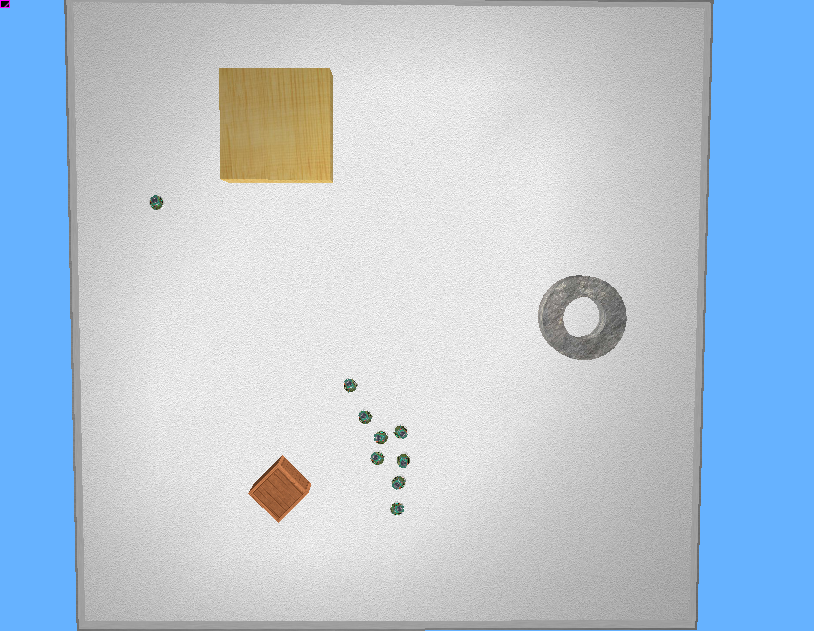
\includegraphics[width=.75\linewidth]{swarm_test_3}
		\caption*{t = 30s}
		\label{fig:sw3}
	\end{minipage}%
	\begin{minipage}{.5\textwidth}
		\centering
		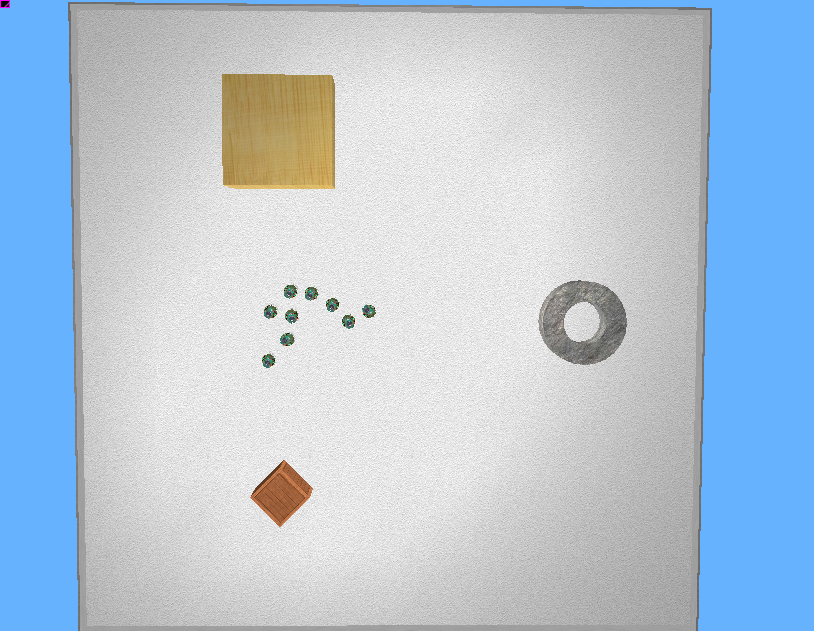
\includegraphics[width=.75\linewidth]{swarm_test_4}
		\caption*{t = 40s}
		\label{fig:sw4}
	\end{minipage}
		\captionof{figure}{Swarm movement over time}
		\label{fig:sw5}
\end{figure}

Figure \ref{fig:sw5} shows the movement of the swarm over a 40 second period. Initially, the robots are separated. As can be seen, at \(t = 10s\), each unit has moved relative to its starting position however do not yet exhibit group behaviour. Soon after this point though, the agents begin to coalesce into a cohesive group. By \(t = 30s\), the majority of agents are within detection range and are moving together. By \(t = 40s\), all of the agents have formed one group, which expand, contract and move around the environment together.

This can be shown graphically (Fig. \ref{fig:exp1}, Fig. \ref{fig:exp1-avg}), through the collection of data directly from the simulated robots. As can be seen, as time increases, the number of robots detected tends to the maximum in the arena.
\clearpage

\begin{sidewaysfigure}
	\centering
\begin{minipage}{1\textwidth}
	\centering
	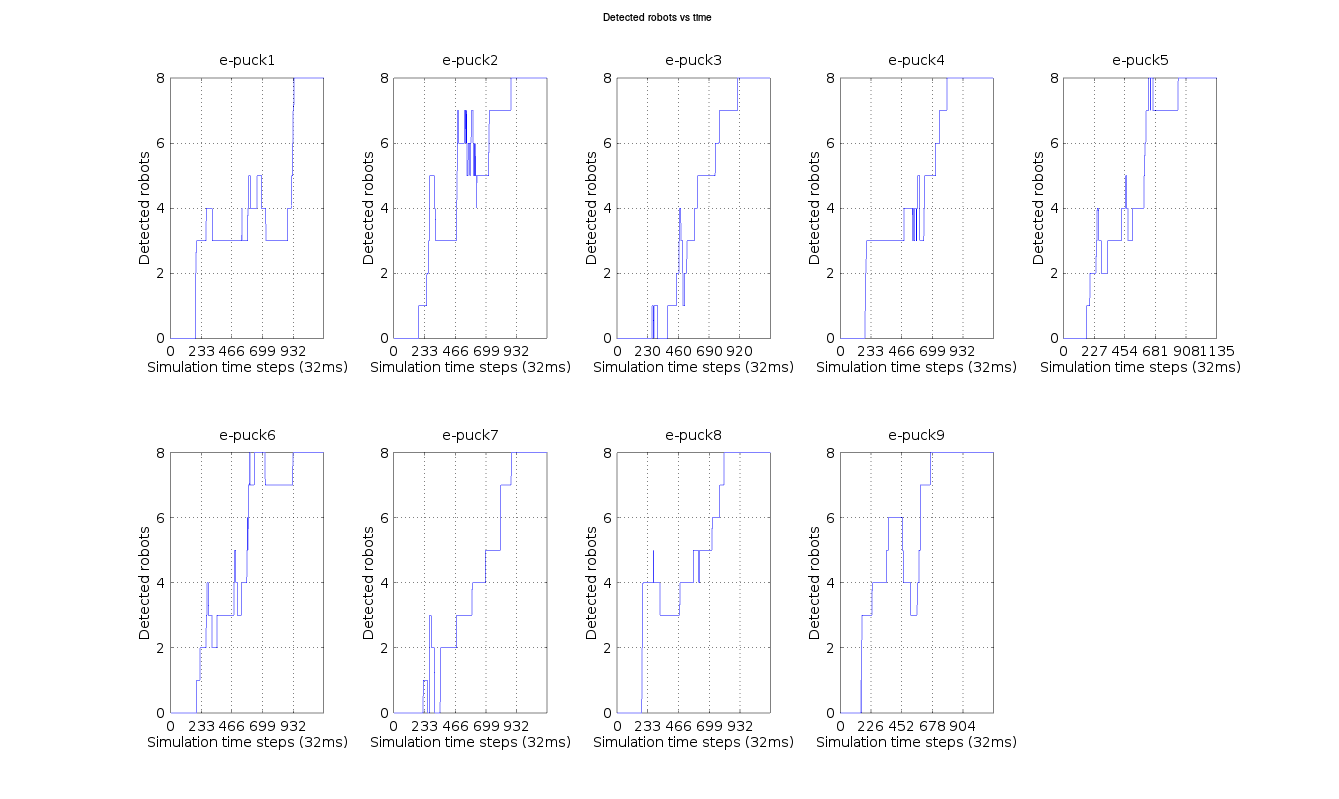
\includegraphics[width=1\linewidth]{data1}
	\captionof{figure}{Number of robots detected vs time}
	\label{fig:exp1}
\end{minipage}%
\end{sidewaysfigure}
\clearpage

\begin{figure}[!t]
		\centering
	\begin{minipage}{1\textwidth}
		\centering
		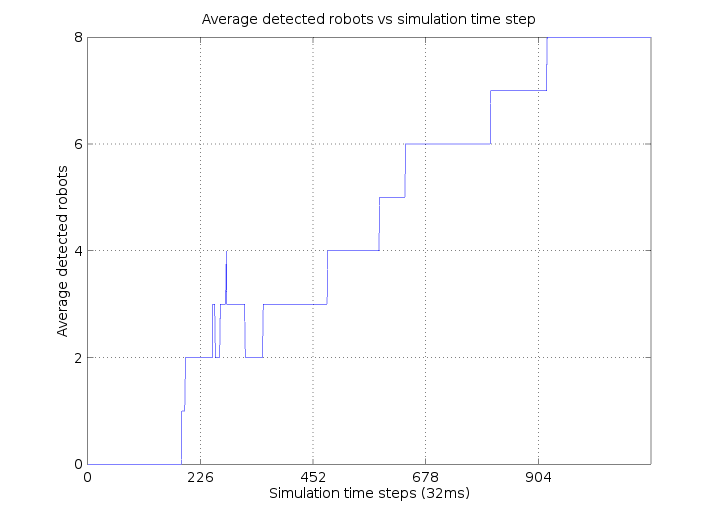
\includegraphics[width=1\linewidth]{data1-average}
		\captionof{figure}{Average number of detected robots}
		\label{fig:exp1-avg}
	\end{minipage}%
\end{figure}

This proves that given enough time, the swarm system will form into one cohesive flock. Due to the nature of the design of the system, there is no higher level supervisor (human or otherwise) co-ordinating the movements of the flock. Therefore, as the system moves to eventually form a group without external aid, the swarm can be said to exhibit self-organization. Furthermore, since each robot broadcasts information locally and does not require any form of positional data detailing the whole swarm, the system can be said to be only interacting locally.

Given the above analysis, this system satisfies \citeauthor{VanDykeParunak2004}'s definition of a swarm, \textit{``useful self-organization of multiple entities through local interactions''} \cite{VanDykeParunak2004}.

Next, the behavioural similarities to natural systems can be examined.

\clearpage

\begin{figure}[h]
	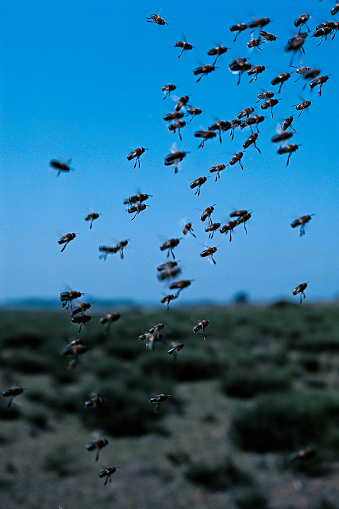
\includegraphics[width=.355\linewidth]{bee-swarm}
	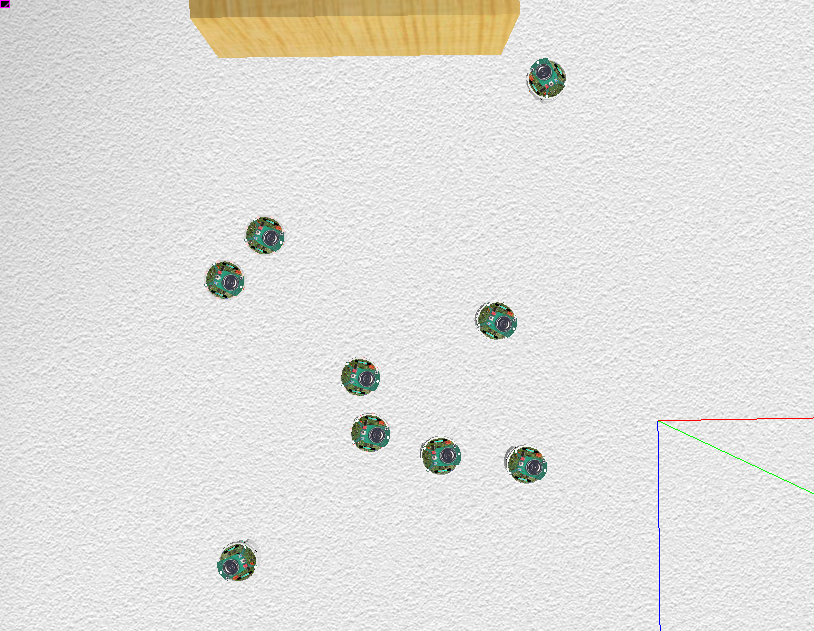
\includegraphics[width=.5\linewidth]{epuck-bees}
	\captionof{figure}{Swarm of bees vs a swarm of e-pucks}
	\label{fig:bees}
\end{figure}

Owing to the e-puck swarm's rapid movements within the swarm boundary, the most similar biological equivalent would be a swarm of bees. As can be seen from Figure \ref{fig:bees}, both systems exhibit strikingly similar behaviour. Both are homogenous groups, forming a loose collective of units. The majority of agents of both groups are oriented to the same heading, with some outliers steering toward the group. 

Through analysis of the above experiment, the question can be answered. The swarm system can be said to be exhibiting flocking and is an example of biologically inspired behaviour.
\clearpage
\subsection{Experiment 2}

\tabulinesep = 1mm
\begin{figure}[!h]
	\centering
	\begin{minipage}{.6\textwidth}
		\centering
		\begin{tabu} to .75\textwidth { | X[c] | X[c] | }
			\hline
			Run & Average time steps (32ms)\\
			\hline
			1 & 920 \\
			\hline
			2 & 380 \\
			\hline
			3 & 1459 \\
			\hline
			4 & 1873 \\
			\hline
			5 & 914 \\
			\hline
			Average & 1109 (35.488s) \\
			\hline
		\end{tabu}
		\caption{Average time steps to aggregation} 	% \caption IS ALWAYS FIRST
		\label{fig:average-time} 	% \label IS ALWAYS SECOND
	\end{minipage}
\end{figure}

In order to answer this question, the average of multiple simulation runs were made. It can be seen from Fig. \ref{fig:average-time} that the average time to aggregation is 35.488 seconds. This is in line with Fig. \ref{fig:sw5}. The wide range in average times can be explained by the randomness of movement that is inherrent in emergent system like this one.

Though the time to aggregation is fast, this can be improved further if a higher level controller is directing the behaviour of every e-puck. However, this would not be a true, decentralised swarm system and would thus be more susceptible to errors and failure.

\clearpage

\subsection{Experiment 3}

\begin{figure}[!h]
	\centering
	\begin{minipage}{.5\textwidth}
		\centering
		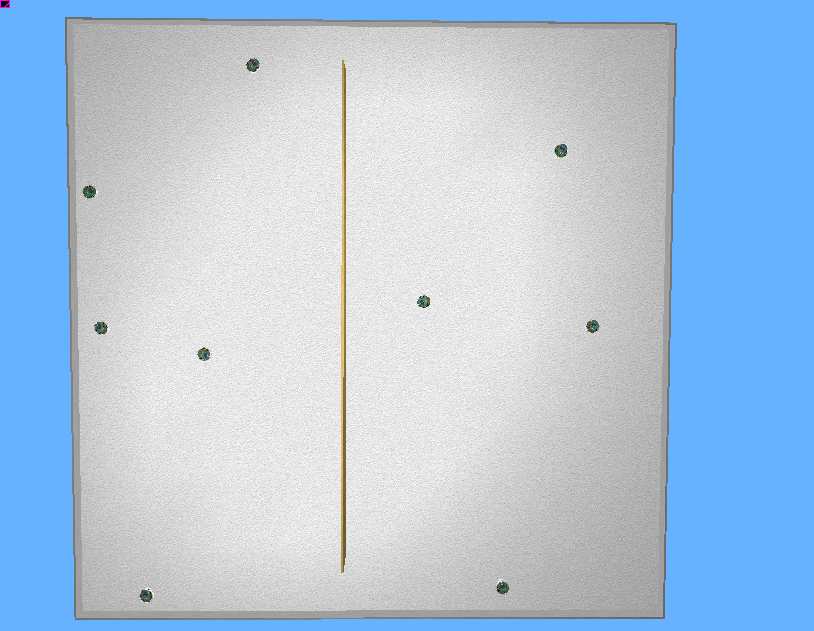
\includegraphics[width=.75\linewidth]{segregate1}
		\caption*{t = 0s}
		\label{fig:seg1}
	\end{minipage}%
	\begin{minipage}{.5\textwidth}
		\centering
		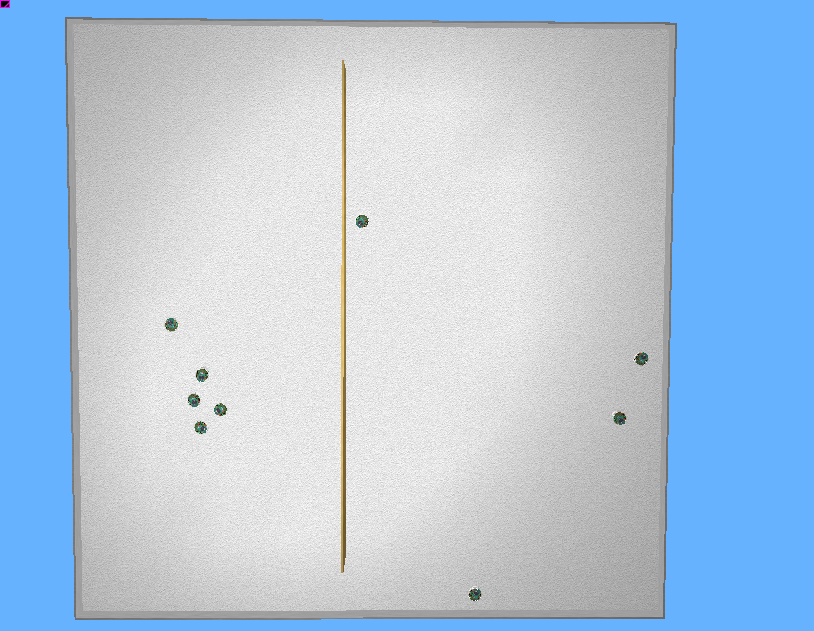
\includegraphics[width=.75\linewidth]{segregate2}
		\caption*{t = 20s}
		\label{fig:seg2}
	\end{minipage}
	\begin{minipage}{.5\textwidth}
		\centering
		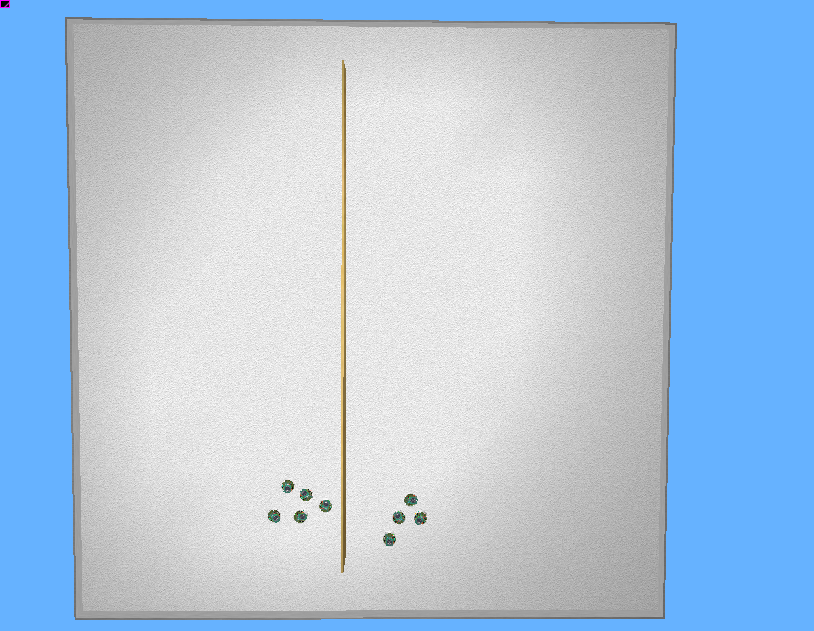
\includegraphics[width=.75\linewidth]{segregate3}
		\caption*{t = 60s}
		\label{fig:seg3}
	\end{minipage}%
	\begin{minipage}{.5\textwidth}
	\centering
	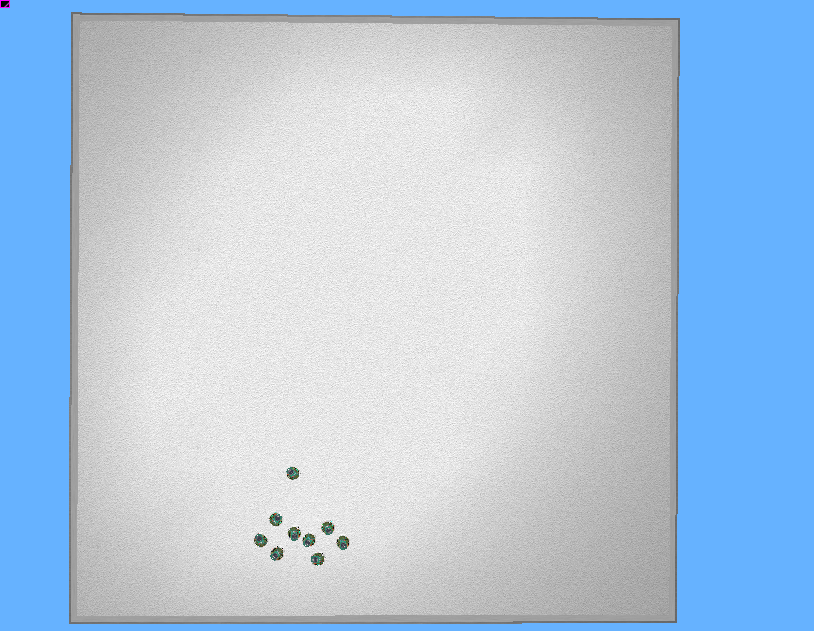
\includegraphics[width=.75\linewidth]{segregate4}
	\caption*{t = 70s}
	\label{fig:seg4}
\end{minipage}%	
	\captionof{figure}{Splinter group test}
	\label{fig:seg}
\end{figure}

Figure \ref{fig:seg} shows the segregated system over a 70 second time period. As predicted, each group on either side of the barrier are quickly able to form independent formations, though the  time taken to do this is increased due to a decrease in swarm density. Once the barrier is removed, the two groups quickly attract one another and amalgamate to form one flock.

This is due to the inherrent locality of the swarm's interactions. Each member of the swarm does not have information on the state of the entire system, thus it behaves according to what is presented to it nearby.

In addition to this, this experiment showed the ability of the swarm to operate in a different and changing environment. Again, this is due to the locality of the agent-agent interactions. This is a demonstration of how crucial the concept of locality is to a swarm's ability to cope with fault tolerance and a dynamic environment.
\clearpage

\subsection{Experiment 4}

\begin{figure}[!h]
	\centering
	\begin{minipage}{.5\textwidth}
		\centering
		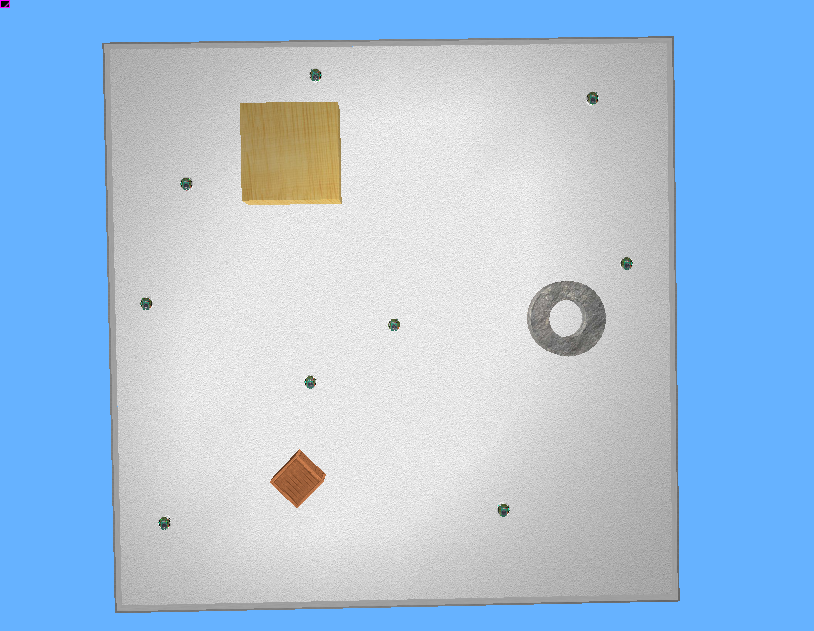
\includegraphics[width=.75\linewidth]{failure1}
		\caption*{t = 0s}
		\label{fig:sfail1}
	\end{minipage}%
	\begin{minipage}{.5\textwidth}
		\centering
		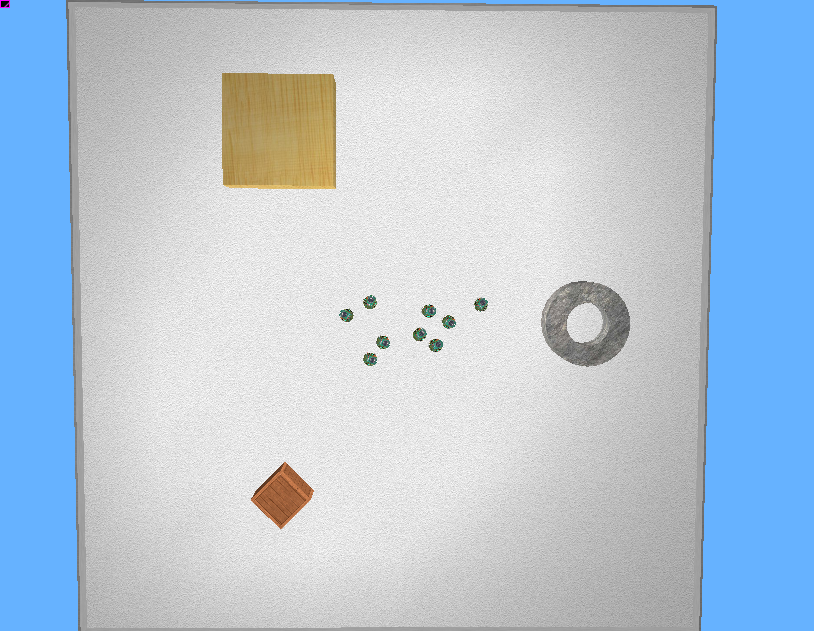
\includegraphics[width=.75\linewidth]{failure2}
		\caption*{t = 35s}
		\label{fig:fail2}
	\end{minipage}
	\begin{minipage}{.5\textwidth}
		\centering
		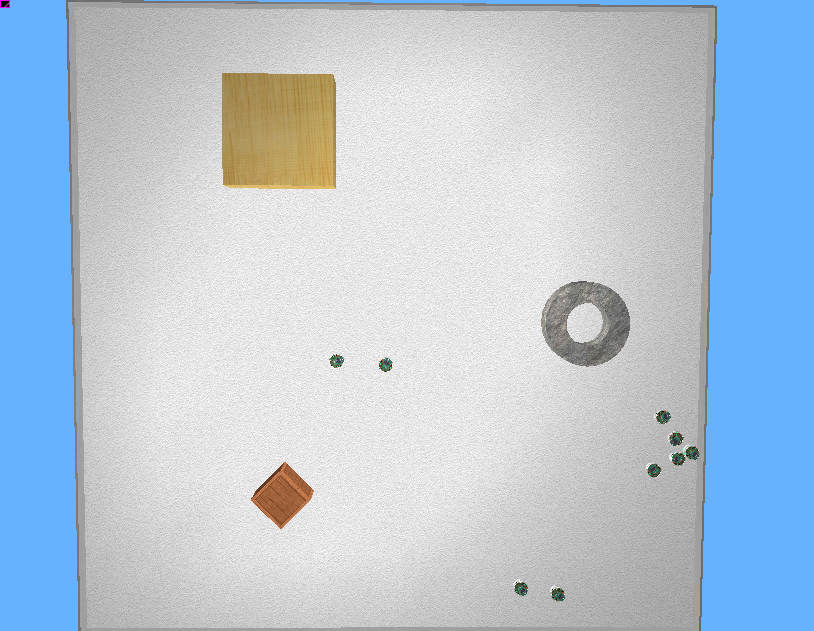
\includegraphics[width=.75\linewidth]{failure3}
		\caption*{t = 180s}
		\label{fig:fail3}
	\end{minipage}%
	\captionof{figure}{Failure test}
	\label{fig:fail}
\end{figure}

The simulation was allowed to progress until a flock had amalgamated, in this case at \(t = 35s\). After this instance, two agents were powered down (e-puck1 and e-puck4, in the center of the arena) to simulate a fatal error/fault. It can be seen in Fig. \ref{fig:fail} that over time, the system ignores these two inoperable robots and continues exhibiting flocking behaviour. 

This is because the functional agents do not receive any signals from the inoperable agents and will treat them as if they were another obstacle in the environment, something to be avoided. 

This can be validated through Fig. \ref{fig:exp4}. As can be seen, all robots bar e-puck1 and e-puck4 settle at detecting 6 robots, which is the total number of functional robots in the swarm.

\begin{sidewaysfigure}
	\centering
	\begin{minipage}{1\textwidth}
		\centering
		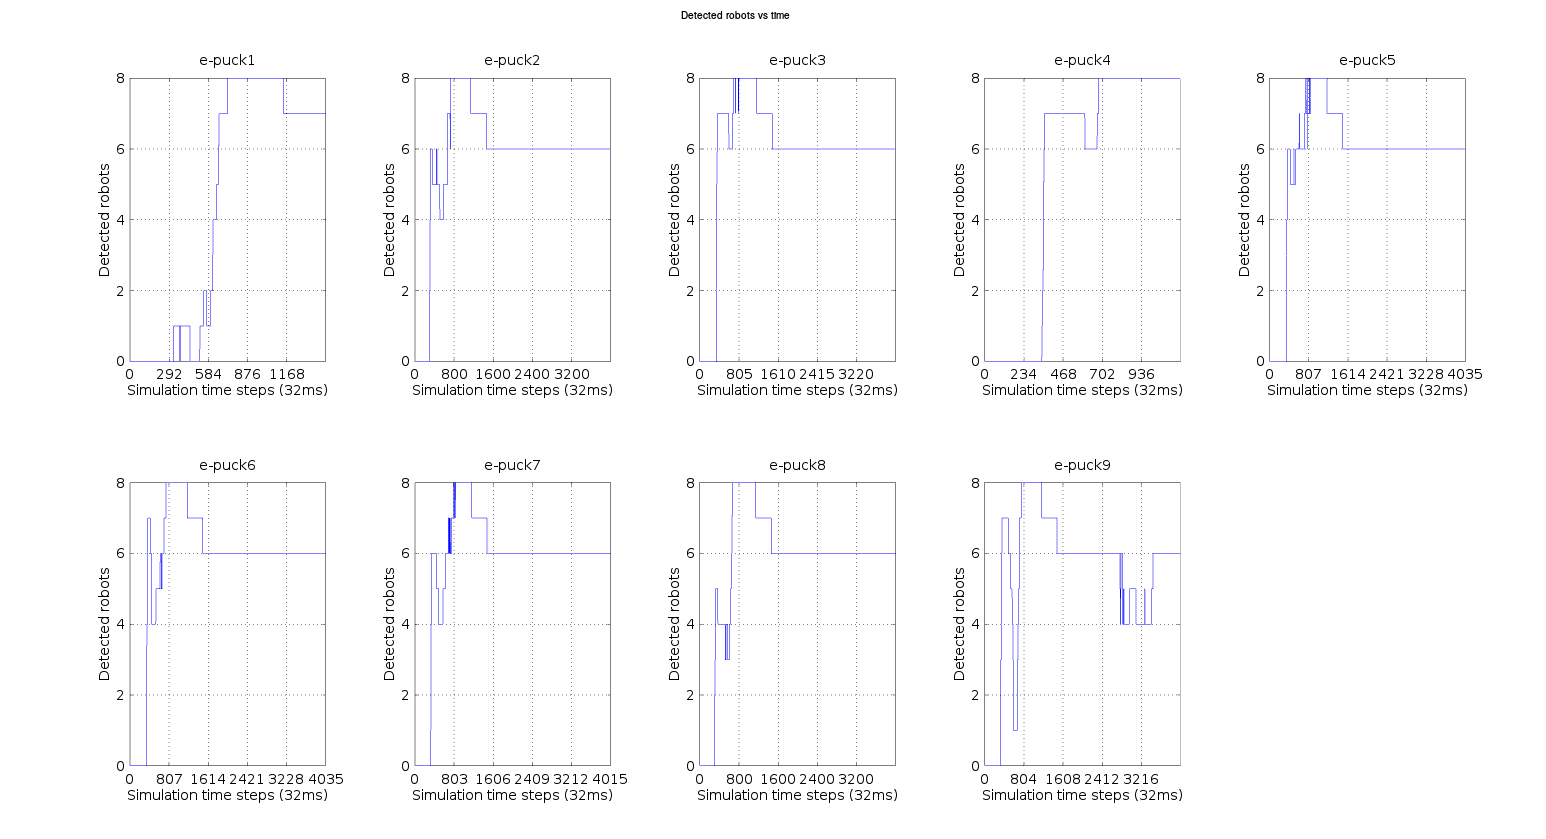
\includegraphics[width=1\linewidth]{data-failure}
		\captionof{figure}{Number of robots detected vs time}
		\label{fig:exp4}
	\end{minipage}%
\end{sidewaysfigure}
\clearpage

\subsection{Experiment 5}

\begin{figure}[!h]
	\centering
	\begin{minipage}{.5\textwidth}
		\centering
		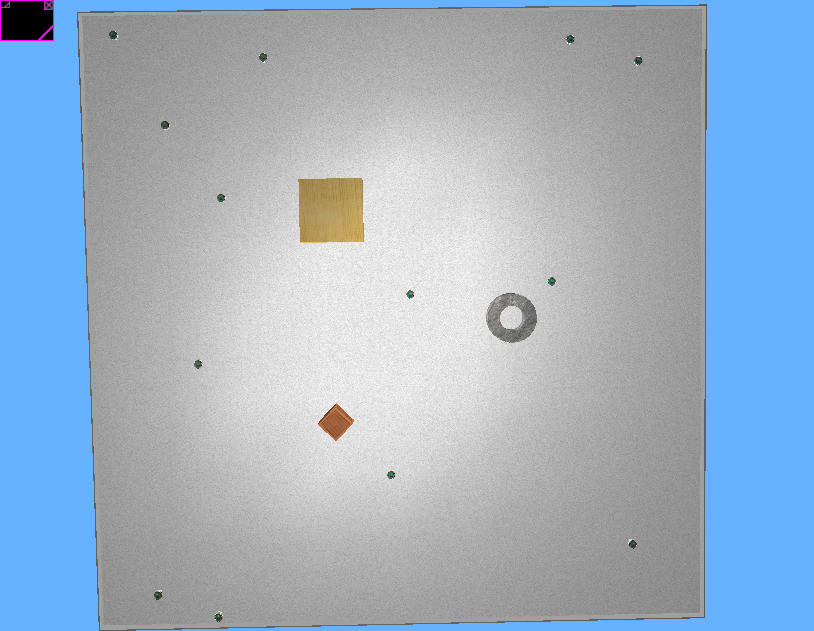
\includegraphics[width=.75\linewidth]{scalable1}
		\caption*{t = 0s}
		\label{fig:scale1}
	\end{minipage}%
	\begin{minipage}{.5\textwidth}
		\centering
		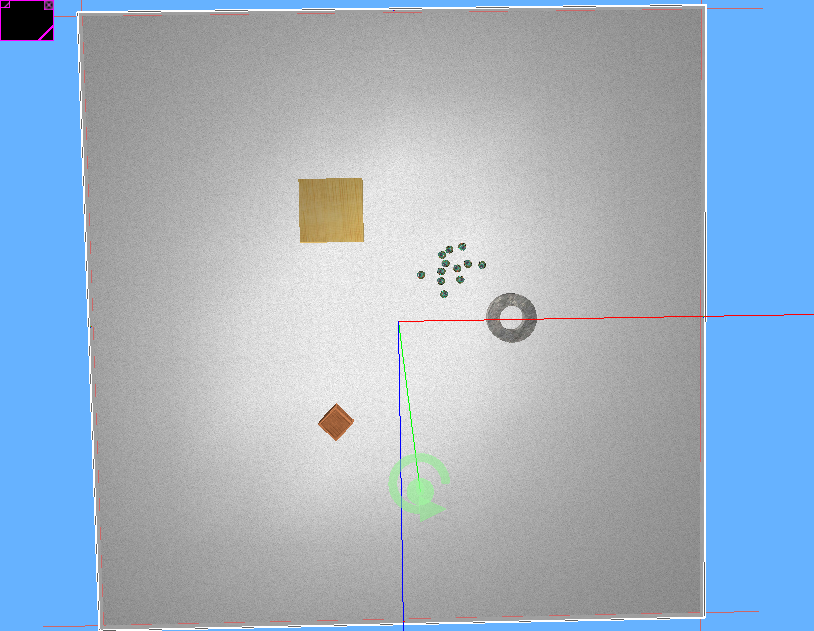
\includegraphics[width=.75\linewidth]{scalable2}
		\caption*{t = 90s}
		\label{fig:scale2}
	\end{minipage}
	\captionof{figure}{Scalability test}
	\label{fig:scale}
\end{figure}

\begin{figure}[h]
	\centering
	\begin{minipage}{1\textwidth}
		\centering
		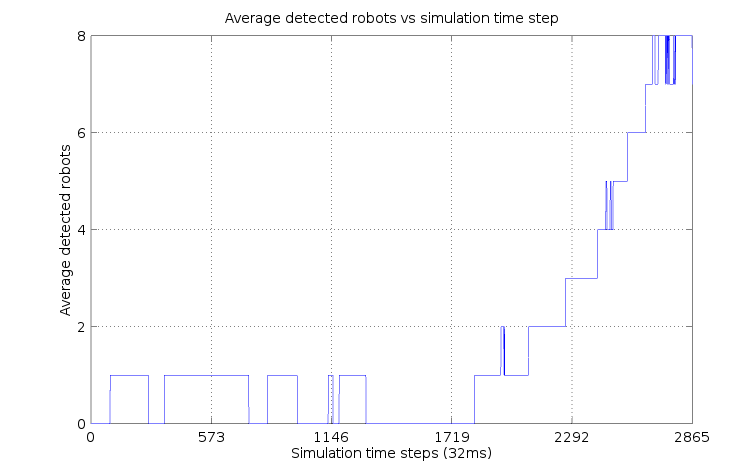
\includegraphics[width=.75\linewidth]{data-scale1}
		\captionof{figure}{Average number of detected robots}
		\label{fig:exp5}
	\end{minipage}%
\end{figure}

Finally, one of the key features of a robot swarm system is its ability to scale in size and still exhibit similar behaviour. 

Along side the swarm's ability to handle errors and faults, Experiment 4 showed how the swarm is capable of scaling \textit{down} in size and still function properly (agent count decreased from 9 to 7). This experiment aimed to shed light on the swarm's ability to scale \textit{up}.

In this case, another 3 agents were introduced to the environment (an increase of 33\%) and the simulation was executed. Shown in Fig. \ref{fig:scale} is a 90 second period of time from the beginning of the simulation. By the end, the swarm had coalesced into a similar formation as shown in previous experiments. 

Once again, this is due to the local nature of the agent-agent interactions. The individual agents do not care about the state of the agents it cannot see nor does it glean any information from a global source.

Adding extra agents to the system does increase the workload that is placed on the simulator, with the simulation running slower than previously. However, this does not effect the behaviour of the robot controller so is ignored. 


\chapter{Conclusion}
\label{chap:Conclusion}

In conclusion, this project set out to study the swarming behaviour exhibited in some biological systems such as social insects, flocks of birds, schools of fish and implement them in an artifical system: a group of mobile robots. It has shown that the application of biologically inspired techniques to the field of swarm robotics can provide interesting and useful results. 

In particular, the rise of emergent self-organisational behaviour within this system satisfies \citeauthor{VanDykeParunak2004}'s definition of a swarm, \textit{``useful self-organization of multiple entities through local interactions''} \cite{VanDykeParunak2004}.

The original objectives of this project were:-

\begin{enumerate}
	\item To understand the theory and concepts behind a swarm system, be they natural or artificial, in order to apply them within an engineering design.
	\item To develop a robot controller which exhibits \textit{flocking} behaviour, based on the techniques of self-organising swarm systems.
	\item To evaluate the developed system under dynamic environmental conditions and stressors.
	%\item To analyse the resulting behaviour and compare the similarity and effectiveness of the controller against other solutions and biological equivalents.
\end{enumerate}

As shown in previous sections, all three objectives were achieved. 

Objective 1 was fulfilled through in depth analysis of current state-of-the-art research within the fields of biologically inspired engineering and collective robotics. This provided a basis for the fundamental knowledge needed to fulfill objective 2, to engineer a swarm system from first principles. 

Objective 2 was fulfilled through the design and implementation of the swarming algorithm detailed in Section \ref{section:code}. One of the significant achievements of this work was the development of a single robot controller to exhibit system wide swarming. The principal biologically inspired techniques used within this controller were the concepts of locality and limited agent-agent communication. As discussed and experimentally proven in Section \ref{chap:Evaluation}, this provides a system that is scalable, tolerant of faults and is capable of self-organisation. In addition to this, having one adaptable controller that can be distributed to as many robots as desired is far more time efficient than developing a bespoke controller for every robot in the swarm.

Objective 3 was achieved through experimental analysis, detailed in Section \ref{section:results}. The system was tested to measure its performance in a variety of environments and conditions. These environments and conditions are typical of those faced by swarms, such as a changing world, agent failure, obstacle avoidance and flock merging. The ability of the system to adequately cope with these stressors is a crucial proof of concept of the applicability of swarming techniques within artificial systems. It would be highly beneficial if these useful traits could be obtained for use in other applications, for example use within a collective of autonomous vehicles.

%There are parallels that can be drawn between the behaviour exhibited by this system and the behaviour exhibited by natural systems such as bees (Fig. \ref{fig:bees}), birds and fish. This is useful 

\section{Problems encountered}

During the course of the project, many technical problems were encountered.

The main problem encountered was dealing with obstacle recognition. Animals or insects that exhibit flocking behaviour are able to distinguish between, for example, a wall and a member of its own species. The simulated e-puck has no way of doing this natively, the proximity sensors simply tell the e-puck how close an object is, and not \textit{what} the object is. In contrast, a real e-puck is able to utilise its proximity sensors as a way of signalling its presence, by broadcasting infra-red light. In order to overcome this problem, the use of an infra-red emitter was decided upon. The e-puck uses this emitter to broadcast its orientation, and in this way, provides a way to signal its presence to other e-pucks.

Leading on from this, the next problem was to provide a method that allows the e-puck to interpret an incoming message packet into actionable information. This problem was overcome through the messaging processing methods detailed in Listing \ref{lst:mess-receive} and \ref{lst:mess-pro}. 

Another issue that arose was determining a suitable method to gather data, especially neighbourhood data. One solution was to graphically measure the emitter ranges of every robot and hence determine how many other robots it detects. Doing this many times over in every simulation would be extremely time consuming and could lead to false results. Instead, it was decided to implement data gathering features within the robot controller itself. The robots automatically write any needed values (such as neighbourhood, orientation and GPS data) to files, for later analysis. Then, a MATLAB script was created that parses these files, extracts the data and plots them. In this manner, plenty of accurate data is gathered.

\section{Limitations}

The main limitation of this work is that the swarm stuggles to move in a similar heading for more than a few seconds, with its movements tending more toward attraction and aggregation. This is due to the fact that no overall goal is presented to the swarm, such as moving to a defined co-ordinate as a group. 

Another limitation was the performance of the simulator itself. Adding more e-pucks to the simulation consumed more computational resources, which decreased the execution time and limited the ability to validate and test the scalability of the swarm.

It was found that the algorithm developed in this project, though inspired by Reynolds' rules \cite{Reynolds:1987:FHS:37402.37406}, was not as effective at providing flocking-like behaviour, though the behaviour exhibited is still similar to some biological systems.

\section{Future work}

This project serves as a case study into the effectiveness of applying biologically inspired techniques to engineering designs and is demonstrated successfully during the course of this project. Mimicking natural systems could provide a number of solutions to problems within industry. 

This work can be extended on several fronts:-

\begin{enumerate}
	\item Using evolutionary robotics techniques such as evolving a neural network (which would act as the robot controller) with a genetic algorithm could provide a more robust controller. This would be at the cost of time and complexity.
	\item Implementing a method of user interaction with the swarm (such as following the user's mouse cursor) would increase the scope of experimental testing and could lead to more cohesive behaviour.
	\item Implementing an ability for the simulation to read parameters contained within files would enable experiments to be run much easier.
	\item Using a radio transmitter instead of infra-red would allow signals to travel through obstacles. This would allow the development of different behaviour.
\end{enumerate} 




%%%%%%%%%%%%%%%%%%%%%%%%%%%%
% BIBLIOGRAPHY
\clearpage
\phantomsection
\addcontentsline{toc}{chapter}{Bibliography}
\bibliography{bib}
%%%%%%%%%%%%%%%%%%%%%%%%%%%%


%%%%%%%%%%%%%%%%%%%%%%%%%%%%
% START APPENDICES
\appendix
%%%%%%%%%%%%%%%%%%%%%%%%%%%%

\chapter{e-puck Specifications}

\subsection{Electronic Systems}

\begin{figure}[!h]
	\begin{minipage}{.75\textwidth}
		\centering
		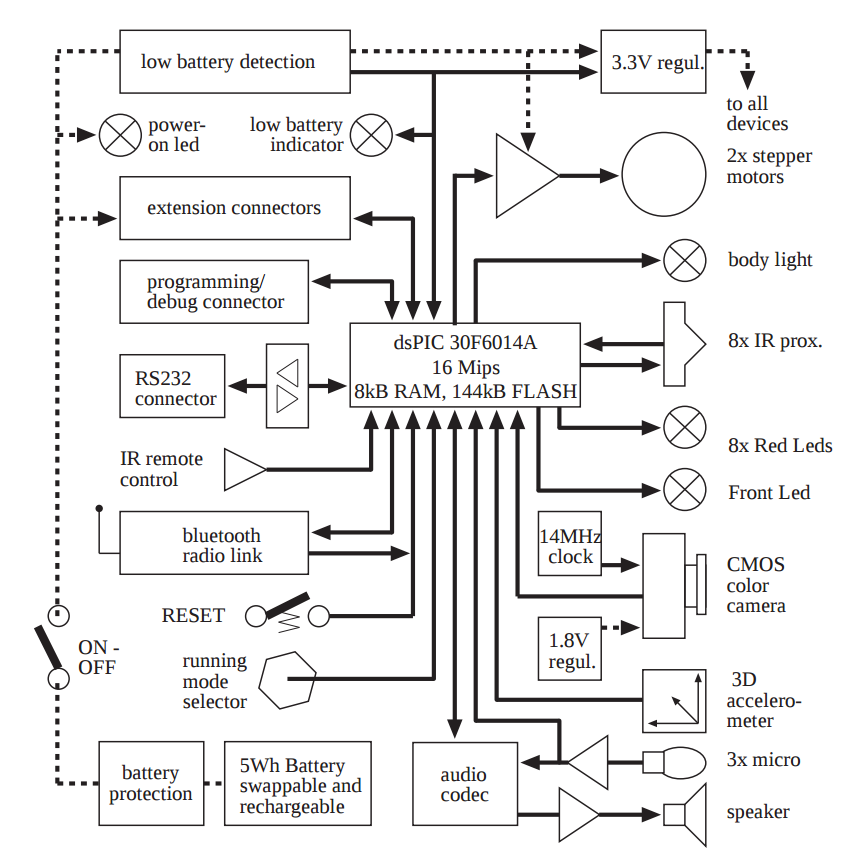
\includegraphics[width=1\linewidth]{electronics.png}
		\captionof{figure}{e-puck electronics systems \cite{epfl-epuck}}
		\label{fig:epuck-elec}
	\end{minipage}
\end{figure}

\clearpage

\subsection{Technical Specifications}
\begin{figure}[]
	\centering
		\begin{minipage}{1\textwidth}
		\centering
\begin{wraptable}{l}{6cm}
	\begin{tabu} to 0.4\textwidth { | X[l] | X[c] | }
		\hline
		Diameter & 7cm \\
		\hline
		Weight & 200g \\
		\hline
		Top speed & 13cm/s \\
		\hline
		Battery & 2 hours \\
		\hline
		Processor & dsPIC 30 CPU @ 30 MHz (15 MIPS) \\
		\hline
		RAM & 8KB \\
		\hline
		Memory & 144KB Flash \\
		\hline
		Motors & Step \\
		\hline
		IR sensors & 8 infra-red proximity and light sensors \\
		\hline 
		Camera & Front facing, 640x480 resolution \\
		\hline
		LEDs & 8 circumferential, 1 body, 1 front \\
		\hline
		Accelerometer & 1, three dimensional \\
		\hline
		Microphones & 3 \\
		\hline
		Speaker & 1 \\
		\hline
	\end{tabu}
	\caption{e-puck specifications} 	% \caption IS ALWAYS FIRST
	\label{fig:tech-specs} 	% \label IS ALWAYS SECOND
\end{wraptable} 
	\end{minipage}
\end{figure}

%-----------------------------------------------------
% Appendix: Code
%-----------------------------------------------------
\chapter{Code}
\label{app:code}

Complete source code can be found at: \url{https://github.com/helmifraser/Swarm}.

%\begin{lstlisting}[language=C++, caption={swarm.hpp},label={lst:swarm-header}]
  // webots libraries
  #include <webots/Camera.hpp>
  #include <webots/Compass.hpp>
  #include <webots/DifferentialWheels.hpp>
  #include <webots/DistanceSensor.hpp>
  #include <webots/Emitter.hpp>
  #include <webots/GPS.hpp>
  #include <webots/Keyboard.hpp>
  #include <webots/LED.hpp>
  #include <webots/LightSensor.hpp>
  #include <webots/Receiver.hpp>
  #include <webots/Robot.hpp>

  // standard libraries
  #include <algorithm>
  #include <array>
  #include <cmath>
  #include <fstream>
  #include <iostream>
  #include <iterator>
  #include <map>
  #include <regex>
  #include <stdio.h>
  #include <stdlib.h>
  #include <string.h>
  #include <thread>
  #include <vector>

  using namespace webots;

  // define the parameters for the simulation and
  #define TIME_STEP 32

  // threshold value for proximity sensors
  #define PS_THRESHOLD 60
  #define WHEEL_SPEED 1000
  #define ARRAY_SIZE 10
  #define SECTOR_ANGLE 45
  #define ALIGN_ERROR 15

  // number of robots to detect before adjustments to steering are made
  #define ALIGN_THRESHOLD 2

  // base emitter range in metres
  #define RANGE 0.35
  #define ROULETTE 7

  struct ReceiverData {
    std::array<int, 6> data{};
    bool received;
    std::array<std::string, ARRAY_SIZE> orientationString;
    std::array<double, ARRAY_SIZE> orientationDouble;
  };


  class Swarm : public DifferentialWheels{
  private:

    // define needed webots objects
    Camera *camera;
    DistanceSensor *distanceSensors[8];
    LED *leds[8];
    DifferentialWheels *diffWheels;
    Emitter *emitter;
    Receiver *receiver;
    Keyboard *keyboard;
    Compass *compass;
    GPS *gps;

    ReceiverData myData;

    std::string robot_name;
    const char *data;

    std::array<int, 3> speed;
    std::array<double, 3> currentOrientation;
    double signalStrength[100];
    double emitterDirection[100][3];
    int multiplier;
    int robots;
    int choose;
    int targetHeading;

    int matrix[100][100];

    double ps_values[8];
    bool left_obstacle, right_obstacle, front_obstacle, back_obstacle;
    bool aligned;

  public:
    Swarm();
    void run();
    void randomAlign();
    int randomVal(int range);
    void objectDetectionMode();
    void teleop();
    void flock();
    void computeDirections(std::array<double, 100> &allDirections);
    void computeCluster(std::array<double, 100> &allDirections, std::array<int, 4> &output);
    int chooseSector(std::array<int, 4> &output);
    bool checkSector(int sector);
    double randomSectorAngle(int sector);
    void adjust(double angle);
    void sendCurrentSpeed();
    void sendCurrentOrientation();
    void getReceiverData();
    void processReceiverData(std::array<std::string, ARRAY_SIZE> data);
    void sendPacket(std::string message);
    void distanceCheck();
    void objectDetection(double speedAdjust);
    void separation();
    void align(int heading);
    int getCurrentHeading();
    int orientationToHeading(int current);
    bool checkAlignment();
    void saveCompassValues();
    std::array<double, 3> getGPSValue();
    double getCurrentOrientation();
    double computeVectorMagnitude(std::array<double, 3> components);
    double computeVectorAngle(std::array<double, 3> components);
    int computeAverageHeading();
    int calculateMode(int array[], int size);
    void keyboardControl(int keyPress);
    int readKey();
    void move(int left, int right);
    void setLEDs(int value);
    double checkDistanceSensor(int n);
    double roundNum(double x);
    std::string printName();

  };
\end{lstlisting}


%\begin{lstlisting}[language=C++, caption={swarm.cpp},label={lst:swarm-header}]
  #include "swarm.hpp"

  Swarm::Swarm() {

    compass = getCompass("compass");
    compass->enable(TIME_STEP);

    gps = getGPS("gps");
    gps->enable(TIME_STEP);

    std::string ps = "ps";
    std::string led = "led";

    for (unsigned int i = 0; i < 8; i++) {
      distanceSensors[i] = getDistanceSensor(ps.replace(2, 1, std::to_string(i)));
      distanceSensors[i]->enable(TIME_STEP);
      leds[i] = getLED(led.replace(3, 1, std::to_string(i)));
    }

    emitter = getEmitter("emitter");
    emitter->setRange(RANGE);
    receiver = getReceiver("receiver");
    receiver->enable(TIME_STEP);

    keyboard = getKeyboard();
    keyboard->enable(TIME_STEP);

    robot_name = getName();
    data = "";

    speed = {100, 50, 0};
    multiplier = 1;

    myData.received = false;
    myData.data[6] = 0;

    robots = 0;
    srand(time(0));
    choose = rand() % 3;
    aligned = false;

    for (int i = 0; i < 100; i++) {
      for (int j = 0; j < 100; j++) {
        matrix[i][j] = 0;
      }
    }

    for (int i = 0; i < 100; i++) {
      for (int j = 0; j < 100; j++) {
        srand(time(NULL) * i + j);
        matrix[i][j] = rand() % 15872567351;
      }
    }
  }

  /* this function waits for a keyboard input to specify which mode the simulation
   *    should run in
   */

  void Swarm::run() {
    std::cout << "1 for keyboard control, 2 for object avoidance, 3 for "
                 "flocking"
              << std::endl;
    std::cout << "Press 5 to stop the simulation. Not doing this will corrupt "
                 "the data output."
              << std::endl;
    while (step(TIME_STEP) != -1) {
      int decide = readKey();
      switch (decide) {
      case 49:
        std::cout << "Keyboard control mode (epuck2)" << std::endl;
        std::cout << "WASDQE keys for control" << std::endl;
        teleop();
        break;
      case 50:
        std::cout << "Object avoidance mode" << std::endl;
        objectDetectionMode();
        break;
      case 51:
        std::cout << "Flock" << std::endl;
        flock();
        break;
      }
    }
  }

  /*
    Flocking algorithm.
    This function provides the swarming behaviour.
    A detailed explanation of which can be found in the Implementation section.
   */

  void Swarm::flock() {

    // creates a robot specific .csv file for outputting data to
    std::string filename = printName() + "_data.csv";
    std::ofstream data(filename, std::ios::out);
    if (data.is_open()) {
      data << printName() << "\n";
      data << "x-value,z-value,robots,orientation\n";
    }

    // spins each robot to a random angle
    randomAlign();

    int quit = 0;
    int step_count = 0;

    // this loop runs infinitely until Webots throws an error or the escape key is
    // pressed
    while (step(TIME_STEP != -1) && quit != 1) {

      getReceiverData();
      processReceiverData(myData.orientationString);

      saveCompassValues();
      distanceCheck();

      int index = std::distance(
          signalStrength,
          std::max_element(signalStrength,
                           signalStrength +
                               sizeof(signalStrength) / sizeof(double)));

      std::array<double, 3> direction = {0, 0, 0};
      if (robots > ALIGN_THRESHOLD) {
        for (int k = 0; k < 3; k++) {
          direction[k] = emitterDirection[index + 1][k];
        }
      } else if (robots == 1) {
        for (int k = 0; k < 3; k++) {
          direction[k] = emitterDirection[index][k];
        }
      }

      double nearestNeighbour = computeVectorAngle(direction);

      /* simple finite state machine arbitration

         If the conditions are right to swarm, robot adjusts its heading.
         Else, move away from any obstacles.

       */

      if ((robots >= ALIGN_THRESHOLD) && (!left_obstacle) && (!right_obstacle) &&
          signalStrength[index] < 10) {
        setLEDs(0);
        adjust(nearestNeighbour);

      } else {
        setLEDs(1);
        objectDetection(1.0);
      }

      double robotsDouble = robots;

      /* Dynamically adaptable range.
         This adds a "gravitational" aspect to a large group, encouraging
         robots to aggregate.
       */

      if (robots >= 1) {
        emitter->setRange(RANGE * (robotsDouble + 1));
      }

      sendCurrentOrientation();
      step_count++;

      int quitKey = readKey();

      switch (quitKey) {
      case 53:
        quit = 1;
        break;

      default:
        break;
      }

      std::array<double, 3> position = getGPSValue();

      if (data.is_open()) {
        data << position[0] << ",";
        data << position[2] << ",";
        data << robots << ",";
        data << getCurrentOrientation() << ",";
        data << " \n";
      }
    }
    move(0, 0);
    data.close();
  }

  void Swarm::randomAlign() {
    int random = randomVal(8);
    while (step(TIME_STEP != -1)) {
      saveCompassValues();
      int test2 = getCurrentHeading();
      if (test2 != random) {
        align(random);
      } else {
        move(0, 0);
        break;
      }
    }
  }

  int Swarm::randomVal(int range) {
    int robNum =
        atoi(robot_name.substr(1, strlen(robot_name.c_str()) - 1).c_str());
    return matrix[robNum][rand() % 100] % range;
  }

  void Swarm::objectDetectionMode() {
    setLEDs(1);
    while (step(TIME_STEP != -1)) {
      objectDetection(1.0);
    }
  }

  void Swarm::teleop() {
    std::string test;
    std::string filename = printName() + "_data_" + test + ".csv";
    std::ofstream data(filename, std::ios::out);

    while (step(TIME_STEP) != -1) {
      if (robot_name.compare("e2") == 0) {
        setLEDs(0);
        // -----get data-----
        int keyPress = readKey();

        saveCompassValues();

        // -----process data-----

        // -----send actuator commands-----
        keyboardControl(keyPress);
        std::array<double, 3> position = getGPSValue();
        std::cout << printName();
        std::cout << "GPS ";
        for (int i = 0; i < 3; i++) {
          std::cout << position[i] << " ";
        }
        std::cout << std::endl;
      }
      if (robot_name.compare("e2") != 0) {
        flock();
        sendCurrentOrientation();
      }
    }
  }

  void Swarm::computeDirections(std::array<double, 100> &allDirections) {
    std::array<double, 3> vector;
    for (int i = 0; i < robots; i++) {
      for (int j = 0; j < 3; j++) {
        vector[j] = emitterDirection[i][j];
      }

      allDirections[i] = computeVectorAngle(vector);
    }
  }

  void Swarm::computeCluster(std::array<double, 100> &allDirections,
                             std::array<int, 4> &output) {

    int countArray[4] = {0, 0, 0, 0};
    // Sorts in ascending order
    std::sort(std::begin(allDirections), std::end(allDirections));

    for (int i = 100 - robots; i < 100; i++) {
      if (allDirections[i] >= 0 && allDirections[i] < 90) {
        countArray[0]++;
      } else if (allDirections[i] >= 90 && allDirections[i] < 180) {
        countArray[1]++;
      } else if (allDirections[i] >= 180 && allDirections[i] < 270) {
        countArray[2]++;
      } else if (allDirections[i] >= 270 && allDirections[i] <= 360) {
        countArray[3]++;
      }
    }

    for (int i = 0; i < 4; i++) {
      output[i] = countArray[i];
    }
  }

  int Swarm::chooseSector(std::array<int, 4> &output) {
    // roulette wheel selection using a fitness function
    int sum = 0;
    std::array<int, 4> outputCopy = output;

    for (int i = 0; i < 4; i++) {
      outputCopy[i] = outputCopy[i] * ROULETTE;
      if (outputCopy[i] == 0) {
        outputCopy[i] = 1;
      }
      sum += outputCopy[i];
    }

    int value = randomVal(sum);
    int i = 0;

    while (value >= 0) {
      value -= outputCopy[i];
      i++;
    }
    i--;

    return i;
  }

  bool Swarm::checkSector(int sector) {
    int myHeading = getCurrentHeading();
    int mySector = 0;

    if ((myHeading >= 0) & (myHeading < 2)) {
      mySector = 1;
    }

    if ((myHeading >= 2) & (myHeading < 4)) {
      mySector = 2;
    }

    if ((myHeading >= 4) & (myHeading < 6)) {
      mySector = 3;
    }

    if ((myHeading >= 6) & (myHeading <= 7)) {
      mySector = 4;
    }

    if (mySector == sector) {
      return true;
    } else {
      return false;
    }
  }

  double Swarm::randomSectorAngle(int sector) {
    double angle = randomVal(90);

    switch (sector) {
    case 0:
      angle += 0;
      break;
    case 1:
      angle += 90;
      break;
    case 2:
      angle += 180;
      break;
    case 3:
      angle += 270;
      break;
    }

    return angle;
  }

  void Swarm::adjust(double angle) {
    double left_speed = WHEEL_SPEED;
    double right_speed = WHEEL_SPEED;

    if (((angle > (360 - ALIGN_ERROR)) & (angle < 360)) |
        ((angle > 0) & (angle < ALIGN_ERROR))) {
      right_speed = left_speed = WHEEL_SPEED;
    } else if ((angle > 270) & (angle < (360 - ALIGN_ERROR))) {
      left_speed =
          (1 + (ALIGN_ERROR + angle - 360) / (90 - ALIGN_ERROR)) * WHEEL_SPEED;
      right_speed = WHEEL_SPEED;
    } else if ((angle >= 180) & (angle < 270)) {
      left_speed = ((angle - 270) / 90) * WHEEL_SPEED;
      right_speed = WHEEL_SPEED;
    } else if ((angle >= 90) & (angle < 180)) {
      right_speed = ((90 - angle) / (90)) * WHEEL_SPEED;
      left_speed = WHEEL_SPEED;
    } else if ((angle >= ALIGN_ERROR) & (angle < 90)) {
      right_speed =
          (1 - (angle - ALIGN_ERROR) / (90 - ALIGN_ERROR)) * WHEEL_SPEED;
      left_speed = WHEEL_SPEED;
    }

    if (left_speed > 1000) {
      left_speed = 1000;
    }

    if (right_speed > 1000) {
      right_speed = 1000;
    }

    move((int)left_speed, (int)right_speed);
  }

  void Swarm::sendCurrentSpeed() {
    std::string message = std::to_string((int)diffWheels->getLeftSpeed()) + " " +
                          std::to_string((int)diffWheels->getRightSpeed());
    sendPacket(message);
  }

  void Swarm::sendCurrentOrientation() {
    std::string message = std::to_string(getCurrentOrientation());
    sendPacket(message);
  }

  void Swarm::getReceiverData() {
    Receiver *copy = (Receiver *)malloc(sizeof(Receiver));
    myData.orientationString = {};
    robots = roundNum((receiver->getQueueLength() + 1) / 2);
    for (int i = 0; i < 100; i++) {
      signalStrength[i] = 0;
    }
    for (int k = 0; k < receiver->getQueueLength(); k++) {
      data = (char *)receiver->getData();
      signalStrength[k] = (double)receiver->getSignalStrength();
      for (int n = 0; n < 3; n++) {
        emitterDirection[k][n] = receiver->getEmitterDirection()[n];
      }
      memcpy(copy, data, sizeof(Receiver));
      myData.orientationString[k] = (char *)copy;
      receiver->nextPacket();
    }
  }

  void Swarm::processReceiverData(std::array<std::string, ARRAY_SIZE> data) {
    myData.received = false;
    for (unsigned int i = 0; i < ARRAY_SIZE; i++) {
      myData.orientationDouble[i] = 0;
    }
    try {
      std::regex re("[*0-9*.*0-9*]+");
      for (int i = 0; i < robots; i++) {
        std::sregex_iterator next(data[i].begin(), data[i].end(), re);
        std::sregex_iterator end;
        while (next != end) {
          std::smatch match = *next;
          std::string match1 = match.str();
          myData.orientationDouble[i] = atoi(match1.c_str());
          if (myData.orientationDouble[i] >= 352) {
            myData.orientationDouble[i] = 0;
          }
          next++;
          if (next == end) {
            myData.received = true;
          }
        }
      }
    } catch (std::regex_error &e) {
    }
  }

  void Swarm::sendPacket(std::string message) {
    std::string temp = printName();
    temp.append(message);
    const char *packet = temp.c_str();
    emitter->send(packet, (strlen(packet) + 1));
  }

  void Swarm::distanceCheck() {
    for (int i = 0; i < 8; i++) {
      ps_values[i] = checkDistanceSensor(i);
    }

    // detect obsctacles
    right_obstacle = (ps_values[0] > PS_THRESHOLD) ||
                     (ps_values[1] > PS_THRESHOLD) ||
                     (ps_values[2] > PS_THRESHOLD);
    left_obstacle = (ps_values[5] > PS_THRESHOLD) ||
                    (ps_values[6] > PS_THRESHOLD) ||
                    (ps_values[7] > PS_THRESHOLD);
    front_obstacle =
        (ps_values[0] > PS_THRESHOLD) & (ps_values[7] > PS_THRESHOLD);
    back_obstacle = (ps_values[3] > PS_THRESHOLD) & (ps_values[4] > PS_THRESHOLD);
  }

  void Swarm::objectDetection(double speedAdjust) {
    distanceCheck();

    double left_speed = speedAdjust * WHEEL_SPEED;
    double right_speed = speedAdjust * WHEEL_SPEED;

    if (!left_obstacle & right_obstacle) {
      left_speed -= speedAdjust * WHEEL_SPEED;
      right_speed += speedAdjust * WHEEL_SPEED;
    } else if (!right_obstacle & left_obstacle) {
      left_speed += speedAdjust * WHEEL_SPEED;
      right_speed -= speedAdjust * WHEEL_SPEED;
    } else if (right_obstacle & left_obstacle) {
      left_speed = -speedAdjust * WHEEL_SPEED;
      right_speed = -speedAdjust * WHEEL_SPEED;
    }

    if (left_speed > 1000) {
      left_speed = 1000;
    }

    if (right_speed > 1000) {
      right_speed = 1000;
    }
    move((int)left_speed, (int)right_speed);
  }

  void Swarm::separation() {
    distanceCheck();

    // init speeds
    double left_speed = WHEEL_SPEED;
    double right_speed = WHEEL_SPEED;

    // modify speeds according to obstacles
    if (left_obstacle | !right_obstacle && !back_obstacle) {
      left_speed = left_speed;
      right_speed = -right_speed;
    } else if (!left_obstacle | right_obstacle && !back_obstacle) {
      left_speed = -left_speed;
      right_speed = right_speed;
    } else if (back_obstacle) {
      left_speed = right_speed = WHEEL_SPEED;
    } else {
      left_speed = right_speed = 0;
    }

    move((int)left_speed, (int)right_speed);
  }

  void Swarm::align(int heading) {

    double target = 0;
    switch (heading) {
    case 0:
      target = 359;
      break;
    case 1:
      target = 45;
      break;
    case 2:
      target = 90;
      break;
    case 3:
      target = 135;
      break;
    case 4:
      target = 180;
      break;
    case 5:
      target = 225;
      break;
    case 6:
      target = 270;
      break;
    case 7:
      target = 315;
      break;
    }
    int current = getCurrentOrientation();
    int max = target + ALIGN_ERROR;
    int min = target - ALIGN_ERROR;
    if (min <= 0) {
      min = 360 - abs(min);
    }

    if ((current >= min) & (current <= max)) {
      move(0, 0);
      aligned = true;
    } else if (current >= max) {
      move(-WHEEL_SPEED, WHEEL_SPEED);
      aligned = false;
    } else if (current <= min) {
      move(WHEEL_SPEED, -WHEEL_SPEED);
      aligned = false;
    }
  }

  int Swarm::getCurrentHeading() {
    int heading = 0;
    int current = getCurrentOrientation();
    if ((current >= (360 - SECTOR_ANGLE / 2)) | (current < (SECTOR_ANGLE / 2))) {
      heading = 0;
    } else if ((current >= SECTOR_ANGLE / 2) & (current < (1.5 * SECTOR_ANGLE))) {
      heading = 1;
    } else if ((current >= (1.5 * SECTOR_ANGLE)) &
               (current < (2.5 * SECTOR_ANGLE))) {
      heading = 2;
    } else if ((current >= (2.5 * SECTOR_ANGLE)) &
               (current < (3.5 * SECTOR_ANGLE))) {
      heading = 3;
    } else if ((current >= (3.5 * SECTOR_ANGLE)) &
               (current < (4.5 * SECTOR_ANGLE))) {
      heading = 4;
    } else if ((current >= (4.5 * SECTOR_ANGLE)) &
               (current < (5.5 * SECTOR_ANGLE))) {
      heading = 5;
    } else if ((current >= (5.5 * SECTOR_ANGLE)) &
               (current < (6.5 * SECTOR_ANGLE))) {
      heading = 6;
    } else if ((current >= (6.5 * SECTOR_ANGLE)) &
               (current < (7.5 * SECTOR_ANGLE))) {
      heading = 7;
    }
    return heading;
  }

  int Swarm::orientationToHeading(int current) {
    int heading = 0;
    if ((current >= (360 - SECTOR_ANGLE / 2)) | (current < (SECTOR_ANGLE / 2))) {
      heading = 0;
    } else if ((current >= SECTOR_ANGLE / 2) & (current < (1.5 * SECTOR_ANGLE))) {
      heading = 1;
    } else if ((current >= (1.5 * SECTOR_ANGLE)) &
               (current < (2.5 * SECTOR_ANGLE))) {
      heading = 2;
    } else if ((current >= (2.5 * SECTOR_ANGLE)) &
               (current < (3.5 * SECTOR_ANGLE))) {
      heading = 3;
    } else if ((current >= (3.5 * SECTOR_ANGLE)) &
               (current < (4.5 * SECTOR_ANGLE))) {
      heading = 4;
    } else if ((current >= (4.5 * SECTOR_ANGLE)) &
               (current < (5.5 * SECTOR_ANGLE))) {
      heading = 5;
    } else if ((current >= (5.5 * SECTOR_ANGLE)) &
               (current < (6.5 * SECTOR_ANGLE))) {
      heading = 6;
    } else if ((current >= (6.5 * SECTOR_ANGLE)) &
               (current < (7.5 * SECTOR_ANGLE))) {
      heading = 7;
    }
    return heading;
  }

  bool Swarm::checkAlignment() {
    bool alignment = false;
    if (getCurrentHeading() == computeAverageHeading()) {
      alignment = true;
    }
    return alignment;
  }

  void Swarm::saveCompassValues() {
    const double *compassVal = compass->getValues();
    for (int i = 0; i < 3; i++) {
      currentOrientation[i] = compassVal[i];
    }
  }

  std::array<double, 3> Swarm::getGPSValue() {
    const double *dataGPS = gps->getValues();
    std::array<double, 3> GPSout;
    for (int i = 0; i < 3; i++) {
      GPSout[i] = dataGPS[i];
    }

    return GPSout;
  }

  double Swarm::getCurrentOrientation() {
    double angle = 360 - computeVectorAngle(currentOrientation);

    return roundNum(angle);
  }

  double Swarm::computeVectorMagnitude(std::array<double, 3> components) {
    double resultant = sqrt(pow(components[0], 2) + pow(components[2], 2));
    return roundNum(resultant);
  }

  double Swarm::computeVectorAngle(std::array<double, 3> components) {
    double x = components[0];
    double z = components[2];
    double angle = 0;
    double pi = 3.141592;

    // Front of robot taken as 0 degrees i.e -z

    if ((x > 0) && (z < 0)) {
      z = -z;
      angle = 90 - atan((z / x)) * 180 / pi;
    } else if ((x > 0) && (z > 0)) {
      angle = 90 + atan((z / x)) * 180 / pi;
    } else if ((x < 0) && (z > 0)) {
      x = -x;
      angle = 180 + (90 - atan((z / x)) * 180 / pi);
    }
    if ((x < 0) && (z < 0)) {
      x = -x;
      z = -z;
      angle = 270 + atan((z / x)) * 180 / pi;
    }

    return roundNum(angle);
  }

  int Swarm::computeAverageHeading() {
    int headings[robots];

    std::array<double, ARRAY_SIZE> copy = myData.orientationDouble;

    if (robots > 0) {
      for (int i = 0; i < robots; i++) {
        if ((copy[i] >= (360 - SECTOR_ANGLE / 2)) |
            (copy[i] < (SECTOR_ANGLE / 2))) {
          headings[i] = 0;
        } else if ((copy[i] >= SECTOR_ANGLE / 2) &
                   (copy[i] < (1.5 * SECTOR_ANGLE))) {
          headings[i] = 1;
        } else if ((copy[i] >= (1.5 * SECTOR_ANGLE)) &
                   (copy[i] < (2.5 * SECTOR_ANGLE))) {
          headings[i] = 2;
        } else if ((copy[i] >= (2.5 * SECTOR_ANGLE)) &
                   (copy[i] < (3.5 * SECTOR_ANGLE))) {
          headings[i] = 3;
        } else if ((copy[i] >= (3.5 * SECTOR_ANGLE)) &
                   (copy[i] < (4.5 * SECTOR_ANGLE))) {
          headings[i] = 4;
        } else if ((copy[i] >= (4.5 * SECTOR_ANGLE)) &
                   (copy[i] < (5.5 * SECTOR_ANGLE))) {
          headings[i] = 5;
        } else if ((copy[i] >= (5.5 * SECTOR_ANGLE)) &
                   (copy[i] < (6.5 * SECTOR_ANGLE))) {
          headings[i] = 6;
        } else if ((copy[i] >= (6.5 * SECTOR_ANGLE)) &
                   (copy[i] < (7.5 * SECTOR_ANGLE))) {
          headings[i] = 7;
        }
      }
    }

    int m, temp, n;
    for (m = 0; m < robots; m++) {
      for (n = 0; n < robots - m; n++) {
        if (headings[n] > headings[n + 1]) {
          temp = headings[n];
          headings[n] = headings[n + 1];
          headings[n + 1] = temp;
        }
      }
    }

    int target = calculateMode(headings, robots);

    return target;
  }

  int Swarm::calculateMode(int array[], int size) {
    int counter = 1;
    int max = 0;
    int mode = array[0];
    int oldMode = mode;
    int oldMode2 = mode;

    for (int i = 0; i < size - 1; i++) {
      if (array[i] == array[i + 1]) {
        counter++;
        if (counter >= max) {
          if (oldMode2 == oldMode) {
            max = counter;
            oldMode = mode;
            mode = array[i];
          } else if ((array[i] != mode) & (array[i] != oldMode)) {
            oldMode2 = array[i];
          }
        }
      } else {
        counter = 1; // reset counter.
      }
    }

    if ((mode != oldMode) & (mode != oldMode2) & (oldMode != oldMode2)) {
      switch (choose) {
      case 0:
        mode = mode;
        break;

      case 1:
        mode = oldMode;
        break;

      case 2:
        mode = oldMode2;
        break;
      }
    }

    return mode;
  }

  void Swarm::keyboardControl(int keyPress) {

    switch (keyPress) {
    // W
    case 87:
      move(multiplier * speed[0], multiplier * speed[0]);
      break;

    // S
    case 83:
      move(-multiplier * speed[0], -multiplier * speed[0]);
      break;

    // A
    case 65:
      move(-multiplier * speed[0], multiplier * speed[0]);
      break;

    // D
    case 68:
      move(multiplier * speed[0], -multiplier * speed[0]);
      break;

    // Q
    case 81:
      move(multiplier * speed[1], multiplier * speed[0]);
      break;

    // E
    case 69:
      move(multiplier * speed[0], multiplier * speed[1]);
      break;

    // UP ARROW
    case 315:
      if (multiplier < 10) {
        multiplier++;
      }
      break;

    // DOWN ARROW
    case 317:
      if (multiplier > 1) {
        multiplier--;
      }
      break;

    default:
      move(multiplier * speed[2], multiplier * speed[2]);
      break;
    }

    std::cout << "Going " << multiplier << " times base speed" << std::endl;
  }

  int Swarm::readKey() { return keyboard->getKey(); }

  void Swarm::move(int left, int right) { setSpeed(left, right); }

  void Swarm::setLEDs(int value) {
    for (int i = 0; i < 8; i++)
      leds[i]->set(value);
  }

  double Swarm::checkDistanceSensor(int n) {
    return distanceSensors[n]->getValue();
  }

  double Swarm::roundNum(double x) { return floor(x * 100 + 0.5) / 100; }

  std::string Swarm::printName() {
    std::string name = "[" + robot_name + "] ";
    return name;
  }

  int main(int argc, char *argv[]) {

    Swarm *robot = new Swarm();
    robot->run();
    delete robot;
    return 0;
  }

\end{lstlisting}



%%%%%%%%%%%%%%%%%%%%%%%%%%%%
% END DOCUMENT
\end{document}
%%%%%%%%%%%%%%%%%%%%%%%%%%%%